% !TeX root = ../../script.tex
\documentclass[../../script.tex]{subfiles}

\begin{document}
\section{Surface Integrals}

In this section we will exclusively look at surfaces in $\realn^3$.

\begin{defi}
    Let $V \subset \realn^2$ be open. A mapping $\phi: V \rightarrow \realn^3$ is said to be a parametrized surface if it is $C^1$ and if 
    $\partial_1 \phi(t), ~\partial_2 \phi(t)$ are linearly independent $\forall t \in V$.
    A subset $S \subset \realn3$ is said to be a regular surface, if there exist:
    \begin{itemize}
        \item open subsets $U_1, \cdots, U_n \subset \realn^3$
        \item open subsets $V_1, \cdots, v_n \subset \realn^2$
        \item mappings $\phi_i: V_i \longrightarrow U_i \cap S$
    \end{itemize}
    such that the $\phi_i$ are parametrized surfaces, bijective and have a continuous $\inv{\phi}$.
    These $S$ are also said to be embedded, two-dimensional manifolds, and the $\phi_i$ are then called maps.
    The collection of all maps $\phi_i$ are called atlas.
    
    $S \subset \realn^3$ is said to be a piecewise regular surface if there exist parametrized surfaces $\phi_1, \cdots, \phi_n$, 
    parametrized paths $\gamma_1, \cdots, \gamma_k$ and points $P_1, \cdots, P_l$ such that 
    \[
        S = \phi_1(V_1) \cup \cdots \cup \phi_n(V_n) \cup \gamma(I_1) \cup \cdots \cup \gamma(I_k) \cup \set{P_1, \cdots, P_l}
    \]
\end{defi}

\begin{eg}
    \begin{enumerate}[(i)]
        \item Consider 
        \begin{align*}
            \phi: (0, \infty) \times \realn &\longrightarrow \realn^3 \\
            (s, t) &\longmapsto (s \cos t, s \sin t, t)
        \end{align*}

        \begin{center}
            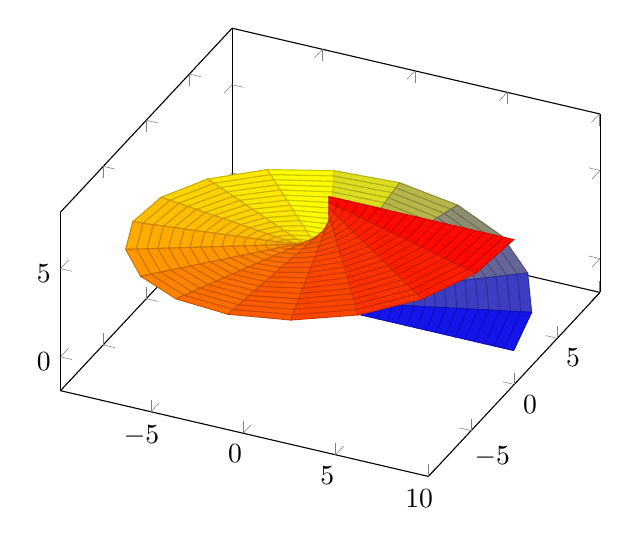
\begin{tikzpicture}
                \begin{axis}[axis equal]
                    \addplot3 [surf, domain=0:10, y domain=0:2*pi, samples=20, z buffer=sort]
                        (
                            {x * cos(y / (2*pi) * 360)}, {x * sin(y / (2*pi) * 360)}, {y}
                        );
                \end{axis}
            \end{tikzpicture}
        \end{center}

        \item The set 
        \[
            S^2 := \set[x^2 + y^2 + z^2 = 1]{(x, y, z) \in \realn^3}
        \]
        is a regular surface. A map describing this surface would be
        \begin{align*}
            \phi: (0, 2\pi) \times (0, \pi) &\longrightarrow \realn^3 \\
            (s, t) &\longmapsto (\cos(s)\sin(t), \sin(s),\sin(t), \cos(t))
        \end{align*}

        \begin{center}
            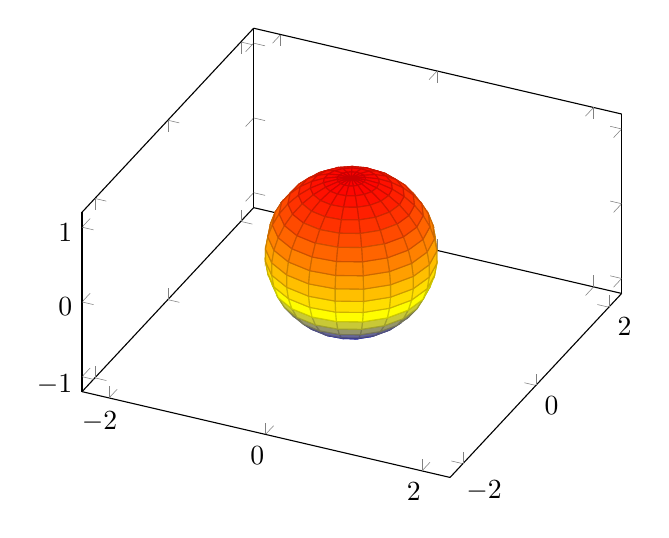
\begin{tikzpicture}
                \begin{axis}[axis equal]
                    \addplot3 [surf, domain=0:360, y domain=0:180, samples=20, z buffer=sort]
                        (
                            {cos(x)*sin(y)}, {sin(x)*sin(y)}, {cos(y)}
                        );
                \end{axis}
            \end{tikzpicture}
        \end{center}

        \item The unit cube 
        \[
            \set[\max\set{\abs{x}, \abs{y}, \abs{z}}]{(x, y, z) \in \realn^3}
        \]
        is a piecewise regular surface.
    \end{enumerate}
\end{eg}

\begin{rem}
    Our definition of regular curves is not equal to the definition of one-dimensional embedded manifolds, because regular curves are not allowed to intersect themselves.
\end{rem}

\begin{defi}[Cross Product]
    Define the vectors $v = (v_1, v_2, v_3)$ and $w = (w_1, w_2, w_3) \in \realn^3$. Then 
    \[
        v \times w = \begin{pmatrix}
            v_2w_3 - v_3w_2 \\ v_3w_1 - v_1w_3 \\ v_1w_2 - v_2w_1
        \end{pmatrix}^T
    \]
    is the cross product of $v$ and $w$.
\end{defi}

\begin{rem}
    \begin{enumerate}[(i)]
        \item The cross product is linear in $v$ and $w$, with 
        \[
            v \times w = w \times v
        \]
        \item $v \times w$ is orthogonal to $v$ and $w$.
        \item The cross product is not associative, but it fulfils the Jacobi-identity:
        \[
            u \times (v \times w) + v \times (w \times u) + w \times (u \times v) = 0
        \]
        \item $v$ and $w$ are linearly dependent if and only if $v \times w = 0$
        \item The definition depends on the coordinates of $v$ and $w$. So the choice of a basis matters. In reality the cross product depends on the scalar product.
        \item Consider the space of anti-symmetric matrices 
        \begin{align*}
            V = \set[A^T = -A]{A \in \realn^{n \times n}} && \dim V = \frac{1}{2} n (n - 1)
        \end{align*}
        The cross product is an outer product on $V$. $V$ can be interpreted as an anti-symmetric bilinear form,
        or as the space of infinitesimal rotations (Lie-algebra to the Lie-group of rotations). This is not relevant.
    \end{enumerate}
\end{rem}

\begin{defi}
    Let $V \subset \realn^2$ be open and $\phi: V \rightarrow \realn^3$ a parametrized surface. Then 
    \[
        \sigma_{\phi}(t) = \partial_1\phi(t) \times \partial_2\phi(t)
    \]
    is said to be a vector surface element of $\phi$, and $\norm{\sigma_{\phi}(t)}$ is the scalar surface element at the point $\phi(t)$.
\end{defi}

\begin{rem}
    The surface element can be defined for arbitrary $C^1$-mappings. $\phi$ is a parametrized surface if and only if 
    $\sigma_{\phi}(t) \ne 0$ or $\norm{\sigma_{\phi}(t)} \ne 0 ~~\forall t \in V$.
\end{rem}

\begin{eg}
    \begin{enumerate}[(i)]
        \item Consider the unit sphere 
        \begin{align*}
            \phi: (0, 2\pi) \times (0, \pi) &\longrightarrow \realn^3 \\
            (s, t) &\longmapsto (\cos(s)\sin(t), \sin(s),\sin(t), \cos(t))
        \end{align*}
        The derivatives of $\phi$ are 
        \begin{align*}
            \partial_1 \phi(s, t) &= (-\sin(t)\sin(s), \sin(t)\cos(s), \cos(t)) \\
            \partial_2 \phi(s, t) &= (\cos(t)\cos(s), \cos(t)\sin(s), -\sin(t))
        \end{align*}
        Then the surface elements are 
        \begin{align*}
            \sigma_{\phi}(s, t) &= (-\sin^2(t)\cos(s), -\sin^2(t)\sin(s), -\sin(t)\cos(t)) \\
            \norm{\sigma_{\phi}(s, t)} &= \sin(t)
        \end{align*}

        \item Let $U \subset \realn^2$ be open, and $f: U \rightarrow \realn$ a continuously differentiable function. Then 
        \[
            \phi(s, t) = (s, t, f(s, t))
        \]
        is a parametrization of the graph of $f$. The derivatives are 
        \begin{align*}
            \partial_1 \phi(s, t) = (1, 0, \partial_1 f(s, t)) && \partial_2 \phi(s, t) = (0, 1, \partial_2 f(s, t))
        \end{align*}
        And the surface elements are 
        \begin{align*}
            \sigma_{\phi}(s, t) &= (-\partial_1 f(s, t), -\partial_2 f(s, t), 1) \\
            \norm{\sigma_{\phi}(s, t)} &= \sqrt{(\partial_1 f(s, t))^2 + (\partial_2 f(s, t))^2 + 1}
        \end{align*}
    \end{enumerate}
\end{eg}

\begin{defi}
    Let $V \subset \realn^2$ be open, $\phi: V \rightarrow \realn^3$ a parametrized surface and $f: \phi(V) \rightarrow \realn$. Then 
    \[
        \iint_{\phi} f \dd{\sigma} := \iint_V f(\phi(t)) \norm{\sigma_{\phi}(t)} \dd{\lambda^2(t)}
    \]
    is said to be the scalar surface integral of $f$ over $\phi$.
    The integral 
    \[
        \iint_{\phi} \dd{\sigma}
    \]
    is said to be the surface of $\phi(V)$.
\end{defi}

\begin{lem}
    Let $V, \tilde{V} \subset \realn^2$ be open, $\phi: V \rightarrow \realn^3$ a parametrized surface and $T: \tilde{V} \rightarrow V$ a diffeomorphismus.
    Set $\psi = \phi \circ T$, then the surface element is 
    \[
        \sigma_{\psi}(t) = \det(DT(t)) \cdot \sigma_{\phi}(T(t))
    \]
\end{lem}
\begin{proof}
    Calculate 
    \begin{equation}
        D\psi(t) = D\phi(T(t)) DT(t)
    \end{equation}
    Or if we consider each column of the derivative separately
    \begin{subequations}
        \begin{equation}
            \partial_1 \psi = \partial_1 T_1 \cdot \partial_2 \phi + \partial_1 T_2 \cdot \partial_2 \phi
        \end{equation}
        \begin{equation}
            \partial_2 \psi = \partial_2 T_1 \cdot \partial_1 \phi + \partial_2 T_2 \cdot \partial_1 \phi
        \end{equation}
    \end{subequations}
    Then 
    \begin{equation}
        \begin{split}
            \sigma_{\psi} = \partial_1 \psi \times \partial_2 \psi &= (\partial_1 T_1)(\partial_2 T_2) \partial_1 \phi \times \partial_2 \phi + (\partial_1T_2)(\partial_2 T_1)\partial_2 \phi \times \partial_1 \phi \\
            &= (\det DT) \sigma_{\phi}
        \end{split}
    \end{equation}
\end{proof}

\begin{rem}
    Let there be the same notation as above, and $f: \phi(V) \rightarrow \realn$
    \begin{align*}
        \iint_{\psi} f \dd{\sigma} &= \iint_{\tilde{V}} f(\psi(t)) \norm{\sigma_{\theta}(t)} \dd{\lambda^2(t)} \\
        &= \iint_{\tilde{V}} f(\phi \circ T(t)) \norm{\sigma_{\psi}(T(t))} \det(DT(t)) \dd{\lambda^2(t)} \\
        &= \iint_V f(\phi(s)) \norm{\sigma_{\phi}(s)} \dd{\lambda^2(s)} = \iint_{\phi} f \dd{\sigma}
    \end{align*}
    In general we have to decompose a (piecewise) regular surface into disjoint regular pieces and parametrize them.
    The surface integral – so the sum of integrals over the pieces – is independent of the chosen decomposition and parametrization.
    Structures of lower dimensions (curves, points) don't contribute to surface integrals.
\end{rem}

\begin{eg}
    \begin{enumerate}[(i)]
        \item We want to calculate the surface of the unit sphere. Using the parametrization we established earlier, we can get 
        \begin{align*}
            \iint_{\phi} \dd{\sigma} = \iint_{(0, 2\pi) \times (0, \pi)} \sin(t) \dd{\lambda^2(s, t)} &= \int_0^{\pi} \int_0^{2\pi} \sin(t) \dd{s}\dd{t} \\
            &= \int_0^{\pi} 2\pi \sin(t) \dd{t} \\
            &= 4\pi
        \end{align*}

        \item Let $U \subset \realn^2$ be open and 
        \begin{align*}
            \phi: U &\longrightarrow \realn^3 \\
            (s, t) &\longmapsto (s, t, 0)
        \end{align*}
        Then $\norm{\sigma_{\phi}} = 1$, and let $f: \realn^2 \times 0 \rightarrow \realn$:
        \[
            \iint_{\phi} f \dd{\sigma} = \iint_U f(s, t, 0) \dd{\lambda^2(s, t)}
        \]
    \end{enumerate}
\end{eg}

\begin{defi}
    Let $V \subset \realn^2$ be open, $\phi: V \rightarrow \realn^3$ a parametrized surface and let $E: \phi(V) \rightarrow \realn^3$. Then 
    \[
        \iint_{\phi} \innerproduct{E}{\dd{\sigma}} := \iint_V \innerproduct{E(\phi(t))}{\sigma_{\phi}(t)} \dd{\lambda^2(t)}
    \]
    is said to be the vector surface integral of $E$ over $\phi$.
\end{defi}

\begin{rem}
    This integral is independent from the parametrization if the determinant $\det DT$ is positive. Then $T$ is said to conserve orientation.
    Otherwise the integral is switching signs.

    For general (piecewise) regular surfaces one has to watch out that the parametrizations are consistent. 
    There are surfaces (regular surfaces even) where that isn't possible (so called non-orientable surfaces).
    For these kinds of surfaces the vector surface integral isn't properly defined.

    If a surface splilts $\realn^3$ into an "outside" and an "inside", then we typically choose the parametrization where the surface elements point outwards.
\end{rem}

\begin{eg}
    We want to integrate 
    \[
        E(x, y, z) := \left(0, 0, \rec{1 + z^2}(x \sin y + y \cos x)\right)
    \]
    over the surface of the unit cube. $E$ points in $z$-direction, so the integrals over the sides disappear.
    So we can parametrize the "lid"
    \[
        (s, t) \longmapsto (s, t, 1) \quad s, t \in [-1, 1]
    \]
    and calculate the integral 
    \[
        \iint \innerproduct{E}{\dd{\sigma}} = \iint_{(-1, 1)^2} \frac{1}{2} (s \sin t + t \cos s) \dd{\lambda^2(s, t)}
    \]
    Doing this for the base yields the same result, just with a different sign.
    So the surface integral over the cube is $0$.
\end{eg}
\end{document}